% Chapter Template

\chapter{Literature review & Overall Description} % Main chapter title

\label{Chapter2} % Change X to a consecutive number; for referencing this chapter elsewhere, use \ref{ChapterX}

\lhead{Chapter 2. \emph{Literature review & Overall Description}} % Change X to a consecutive number; this is for the header on each page - perhaps a shortened title

%----------------------------------------------------------------------------------------
%	SECTION 1
%----------------------------------------------------------------------------------------

\section{LITERATURE REVIEW}

Blind people may not be able to assess far obstacles effectively and have to be constantly aware of surroundings.

\section{Review of Related Work}
The iPhone application for counting the sheets of cloth applies image processing technique to provide the acceptable result. From survey, there are projects that use image processing techniques to count item that is placed overlay. The first project is “Method of Counting Thin Steel Plates Based on Digital Image Processing” proposed by Jingting Li and his team\cite{Method} that uses image processing to prepare the image and draws green straight lines before counting. The second project is “Machine Vision System for Counting the Number of Corrugated Cardboard proposed by Chatchai Suppitaksakul and his team \cite{Machine} that uses image processing to prepare and mark center of corrugated cardboard.\\
\begin{figure}[t]
	\centering
	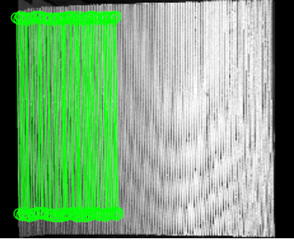
\includegraphics[scale=0.8]{f201.png}
	\caption{Edge detection}
	\label{fig:f201}
\end{figure}
\begin{figure}[t]
	\centering
	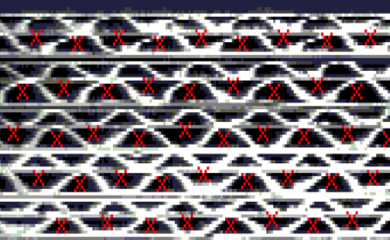
\includegraphics[scale=0.8]{f202.png}
	\caption{Center marking obtain from blob analysis operation}
	\label{fig:f202}
\end{figure}

\textbf{Method of Counting Thin Steel Plates Based on Digital Image Processing}
by Jingting Li and his team.\cite{Method} This project applied the method that offers a way to count piled thin steel plate for car chassis based on digital image processing and software designed for it. First, the image of the piled steel plates was enhanced quality. Then acquiring the region of interest (ROI) and detecting the lines with edge detection, horizontally shear the image against the tilting angle to adjust to vertical. Finally, count the number of plates in a Figure \ref{fig:f201} by counting peaks that count with green lines. The method requires no large mechanical equipment and is efficient and accuracy.\\

\textbf{Machine Vision System for Counting the Number of Corrugated Cardboard}
by Chatchai Suppitaksakul and his team \cite{Machine}. This project presented a method for counting the number of corrugated cardboard that used machine vision system and image processing techniques. The cardboard edge images that were strip or slitter and fluted or cut-off side were used for detection and counting. The gray level of edge images which obtained from the line scan camera were converted to binary images using threshoding. After that the strip lines of the slitter side were extracted by the first-order derivative and morphology then processed with mode for counting. For the cut-off side, the fluted areas of cardboard were identified and measured using Blob analysis. Then the centers of the detected area were marked with red ‘x’ and counted as the number of cardboards as shown in a Figure \ref{fig:f202}. MATLAB was applied to simulate in the experiments for determining the algorithms and performed the real-time experiments using HALCON to see the accuracy and performance of the system. The cardboard type BC, C and B were used in the tests. As experimental results, it is shown that the system provided the correct counting with tolerance of 2 cm and 3 cm in the case of the cardboard placed away further the camera focus for the slitter and cut-off side respectively.


These researches are useful for studying and understanding some techniques that can be applied to our project. Some techniques of aforementioned research are used to implement and solve in our project. Such as center making or centroid, edge detection, etc. 
